\subsection{问题四分析}
问题四旨在提出对某些往返于机场短途载客的出租车司机们的``优先权''方案,本文参考上海浦东国际机场现使用的出租车智能匹配管理系统,考虑定位技术与绩效补贴两方向,同时为短途载客司机们提供``优先权''。

\subsection{大型交通枢纽出租车智能匹配管理系统}
\subsubsection{Beckmann交通分配数学模型}
交通分配模型的变量与参数表示如下:
\begin{itemize}
    \item $x_a$:路段$a$的交通流量,组成向量为$x = (\dots,x_a,\dots)$;
    
    \item $t_a$:路段$a$的交通阻抗;
    
    \item $t_a(x_a)$:以流量为自变量的阻抗函数;
    
    \item $f_k^{rs}$:点对$(r,s)$间第k条路径的交通流量;
    
    \item $C_k^{rs}$:点对$(r,s)$的第$k$条路径阻抗;
    
    \item $u_{rs}$:$(r,s)$的最小阻抗;
    
    \item $\delta_{a,k}^{rs} = \begin{cases}
            1 & \text{路段$a$在$(rs)$间的第$k$条路径}\\
            0 & \text{其他情况};
        \end{cases}$
    
    \item $W_{rs}$:$(r,s)$间的所有路径集合;
    
    \item $q_{rs}$:$(r,s)$间的交通量。
\end{itemize}

\begin{theobox}{系统最优原理}{sysOptimize}
    在交通网络中的交通量应按某种方式分配,以使网络中所有交通元的总阻抗最小。
\end{theobox}

系统最优原理的目标函数是使得网络中所有用户阻抗最小,即:
\begin{equation}\label{eq:最小用户阻抗}
    \begin{aligned}
        & \min: Z(x) = \sum_{a}x_{a}t_{a}(x_a) \\
        & \text{s.t.} \begin{cases}
            \sum_{k}f_{k}^{rs} = q_{rs} & \forall r,s; \\
            f_{k}^{rs} > 0 & \forall r,s,k; \\
            x_a = \sum_{r,s}\sum_k f_{k}^{rs}\dot\delta_{a,k}^{rs} & \forall a.
        \end{cases}
    \end{aligned}
\end{equation}
该系统称为系统最优模型(SO, System Optimization)。

\subsubsection{常见通信系统}
\begin{itemize}
    \item GSM(Global System for Mobile Communications),提供短信。
    
    \item GPRS(General Packet Radio System),介于2G与3G间的通信技术。它具有保持永远在线,按数据流量计费,自如切换、高速传输等优点。
    
    \item GPS(Global Positioning System),广泛应用、高精度。
    
    \item GIS(Geographic Information System),空间数据处理技术;与GPS、RS统称3S系统。
\end{itemize}

\subsection{短途往返出租车司机``优先权''设定}
\subsubsection{发放``智能短途票''}
传统纸质短途票发放给从机场接客且能在一个小时内或规定时间返回机场再次接客的出租车司机,以便该司机下一次返回接客时无需排队,节省等待时间成本。而纸质短途票存在票面日期被随意修改、伪造等问题,人工不易管理。

现今国内其他机场可参考上海浦东机场推行的智能化匹配管理系统,实现短途票电子到账;每部出租车均需安装GPS,以便清楚直观地看到司机是否在一定时间内``短途'',避免弄虚作假,且提高了出租车的运营效率。

\subsubsection{实行多次短途司机的奖励政策}
奖励政策具体草拟如下:

\begin{enumerate} % \begin{enumerate}
    \item 设置司机当日往返机场载客的下界次数$l$与上限$L$,上下界具体数值需依据该机场实际承载旅客量、机场周边路况等因素设置。
    
    \item 依据边际回报递减原理,令司机往返载客次数与奖金提成回报关系满足logistic函数。如图~\ref{fig:logistic}所示,$m,M$分别为奖金数的上下界,$l,L$分别为当日往返机场载客的下上限次数,点$(x_0,y_0)$为该函数段中导数最大的点。
    
    \item 导数最大即意味着边际收益最大,因此可推断出大多数司机的日往返机场载客数趋于$x_0$次,此时大部分司机的回报为$y_0$。此方案一方面能用奖金激励司机短途载客,保障了机场乘车乘客的接机需求;另一方面因接机次数存在上限及边际收益回报递减,能有效地控制司机日往返机场次数,保障了机场周边道路交通的通畅性。
\end{enumerate}

\begin{figure}
    \centering
    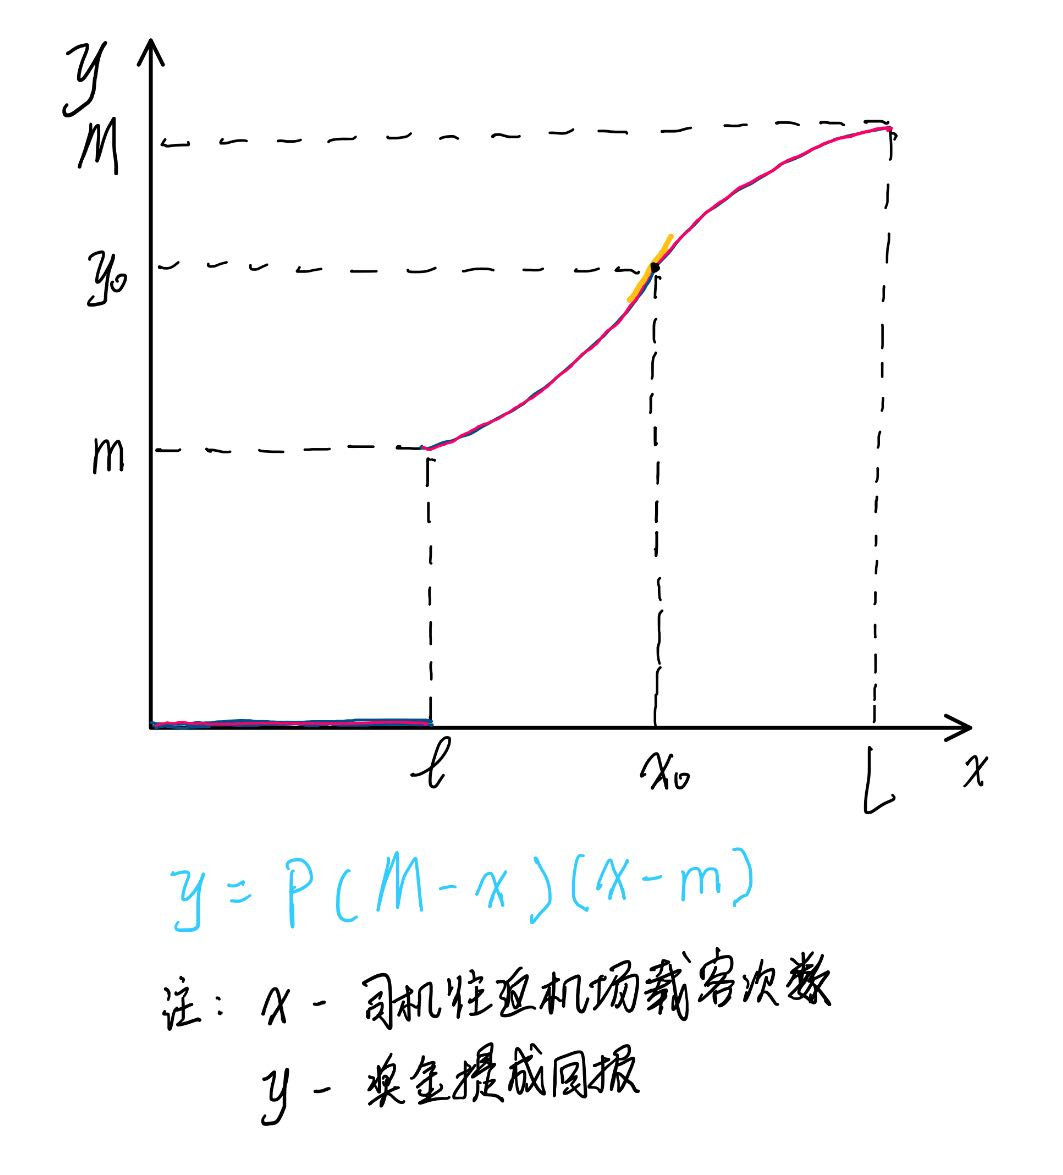
\includegraphics[width=.6\textwidth]{figures/logistic.jpg}
    \caption{司机日往返机场次数与提成回报的关系}
    \label{fig:logistic}
\end{figure}

本文建议采取电子短途票与短途接送奖励政策的同步推进,且此种方案不受机场类型、地域的影响,适宜在全国大范围推广。